\documentclass[]{beamer}
%\documentclass[notes]{beamer}       % print frame + notes
%\documentclass[notes=only]{beamer}   % only notes
%\documentclass{beamer}              % only frames
%\documentclass[handout]{beamer}
\usepackage{tikz}

\usepackage{algorithm2e}

\usetheme{Dresden}%%%%% developer's preference - may change based on preferences

%%%%%% UMass official color: https://www.umass.edu/brand/elements/color
\definecolor{UMassAmherst}{rgb}{0.533 0.11 0.11}
\usecolortheme[named=UMassAmherst]{structure}

\title{Algoritmos}
\subtitle{Divide y Vencer\'as}
\author{MSc Edson Ticona Zegarra}
\institute{Campamento de Programaci\'on}
\date{}

%%%%%% obtained from: https://www.umass.edu/brand/elements/wordmarks-seal-and-spirit-marks
%%%%%% logos of other departments can also be obtained from the above link. Otherwise, consult your department website.

\begin{document}

\maketitle

\begin{frame}{Contenido}
\tableofcontents
\end{frame}

\section{Divide y Vencer\'as}
\begin{frame}{Contenido}
\tableofcontents[currentsection]
\end{frame}

\begin{frame}{Divide y Vencer\'as}
  \begin{itemize}
    \item Es una t\'ecnica de dise\~no de algoritmos en la cual dividimos un problema de tama\~no $n$ en $a$ subproblemas de tama\~no $n/b$
      \pause
    \item Luego, se resuelve recursivamente cada subproblema
      \pause
    \item Finalmente, se combina la soluci\'on a cada subproblema para obtener la soluci\'on al problema inicial
  \end{itemize}
\end{frame}

\begin{frame}{Complejidad}
  \begin{itemize}
    \item $T(n) = a*T(n/b) + T(f(n))$
      \pause
    \item Donde $f(n)$ representa el tiempo necesario para combinar los subproblemas
  \end{itemize}
\end{frame}

\section{Problemas}
\begin{frame}{Contenido}
\tableofcontents[currentsection]
\end{frame}

\begin{frame}{Envolvente convexa: Convex Hull}
  \begin{definition}
    Dado un conjunto de puntos $P$ en el plano, se busca un subconjunto que define la envolvente convexa.
  \end{definition}
  \pause
  \begin{itemize}
    \item Existen varios algoritmos para resolver este problema, ahora nos enfocamos en la soluci\'on divide y vencer\'as
      \pause
    \item La envolvente convexa es el pol\'igono de menor \'area que contiene todos los puntos y lo representamos por CH(P)
  \end{itemize}
\end{frame}

\begin{frame}{Envolvente convexa: Convex Hull}
  \begin{tikzpicture}
    \def\us{(0,2),(1,4),(2,0),(3,2),(4,0),(1,2),(6,2),(5,4)}
    \foreach \u [count=\i from 1] in \us {\node[circle] (u\i) at \u [below] {$p_\i$};}
    \foreach \u [count=\i from 1] in \us {\draw[fill=black] \u circle[radius=1.5pt];}
  \end{tikzpicture}
\end{frame}

\begin{frame}{Envolvente convexa: Convex Hull}
  \begin{tikzpicture}
    \def\us{(0,2),(1,4),(2,0),(3,2),(4,0),(1,2),(6,2),(5,4)}
    \foreach \u [count=\i from 1] in \us {\node[circle] (u\i) at \u [below] {$p_\i$};}
    \foreach \u [count=\i from 1] in \us {\draw[fill=black] \u circle[radius=1.5pt];}
    %For Test
    \draw (u1.north)--(u2.north)--(u8.north)--(u7.north)--(u5.north)--(u3.north)--(u1.north);
  \end{tikzpicture}
\end{frame}

\begin{frame}{Envolvente convexa: Convex Hull}
  \begin{algorithm}[H]
    \SetKwInOut{Input}{input}\SetKwInOut{Output}{output}
    \Input{$P$ es el conjunto de $n$ puntos}
    \Output{$S$ conjunto de puntos representando la envolvente convexa}
    \BlankLine
    $Sort(P)\ por\ x$ \;
    $Left, Right \leftarrow Dividir\ P\ por\ la\ mitad$\;
    $A \leftarrow ConvexHull(Left) $ \;
    $B \leftarrow ConvexHull(Right) $ \;
    $S \leftarrow Combinar\ A\ con\ B$ \;
    \KwRet{$S$}
  \end{algorithm}
\end{frame}

\begin{frame}{Envolvente convexa: Convex Hull}
  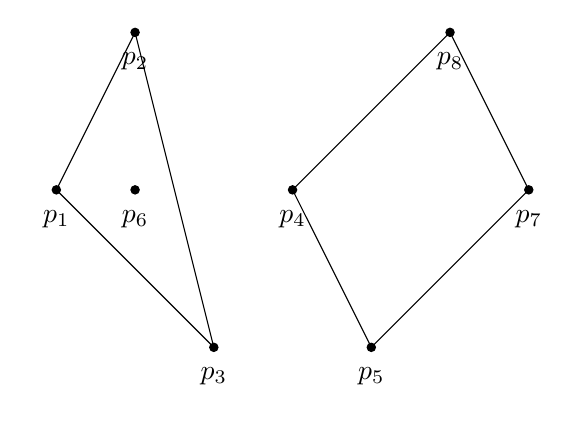
\begin{tikzpicture}
    \def\us{(0,2),(1,4),(2,0),(3,2),(4,0),(1,2),(6,2),(5,4)}
    \foreach \u [count=\i from 1] in \us {\node[circle] (u\i) at \u [below] {$p_\i$};}
    \foreach \u [count=\i from 1] in \us {\draw[fill=black] \u circle[radius=1.5pt];}
    \draw (u1.north)--(u2.north)--(u3.north)--(u1.north);
    \draw (u8.north)--(u7.north)--(u5.north)--(u4.north)--(u8.north);
  \end{tikzpicture}
\end{frame}

\begin{frame}{Envolvente convexa: Convex Hull}
  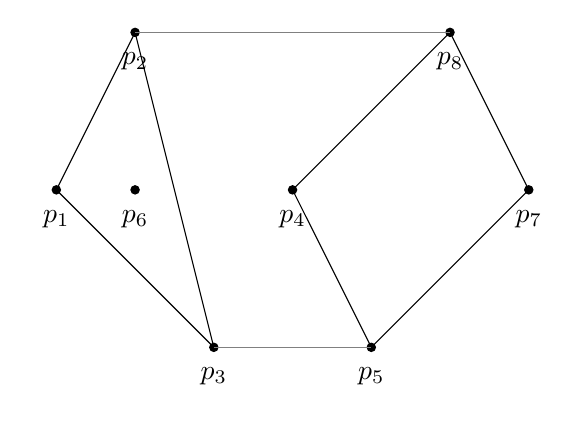
\begin{tikzpicture}
    \def\us{(0,2),(1,4),(2,0),(3,2),(4,0),(1,2),(6,2),(5,4)}
    \foreach \u [count=\i from 1] in \us {\node[circle] (u\i) at \u [below] {$p_\i$};}
    \foreach \u [count=\i from 1] in \us {\draw[fill=black] \u circle[radius=1.5pt];}
    \draw (u1.north)--(u2.north)--(u3.north)--(u1.north);
    \draw (u8.north)--(u7.north)--(u5.north)--(u4.north)--(u8.north);
    \draw[gray] (u2.north)--(u8.north);
    \draw[gray] (u3.north)--(u5.north);
  \end{tikzpicture}
\end{frame}

\begin{frame}{Envolvente convexa: Convex Hull}
  \begin{tikzpicture}
    \def\us{(3,1),(2,3),(1,4),(-1,2),(-2,0),(1,0),(6,4),(6.7,5),(8,5),(9,4),(8,3),(7,3)}
    %         1      2    3     4       5       6    7     8     9    10    11   13
    \foreach \u [count=\i from 1] in \us {\node[circle] (u\i) at \u [below] {$p_{\i}$};}
    \foreach \u [count=\i from 1] in \us {\draw[fill=black] \u circle[radius=1.5pt];}
    \draw (u1.north)--(u2.north)--(u3.north)--(u4.north)--(u5.north)--(u6.north)--(u1.north);
    \draw (u7.north)--(u8.north)--(u9.north)--(u10.north)--(u11.north)--(u12.north)--(u7.north);
  \end{tikzpicture}
\end{frame}

\begin{frame}{Envolvente convexa: Convex Hull}
  \begin{tikzpicture}
    \def\us{(3,1),(2,3),(1,4),(-1,2),(-2,0),(1,0),(6,4),(6.7,5),(8,5),(9,4),(8,3),(7,3)}
    %         1      2    3     4       5       6    7     8     9    10    11   13
    \foreach \u [count=\i from 1] in \us {\node[circle] (u\i) at \u [below] {$p_{\i}$};}
    \foreach \u [count=\i from 1] in \us {\draw[fill=black] \u circle[radius=1.5pt];}
    \draw (u1.north)--(u2.north)--(u3.north)--(u4.north)--(u5.north)--(u6.north)--(u1.north);
    \draw (u7.north)--(u8.north)--(u9.north)--(u10.north)--(u11.north)--(u12.north)--(u7.north);
    \draw[green] (u1.north)--(u7.north);
  \end{tikzpicture}
\end{frame}

\begin{frame}{Envolvente convexa: Convex Hull}
  \begin{tikzpicture}
    \def\us{(3,1),(2,3),(1,4),(-1,2),(-2,0),(1,0),(6,4),(6.7,5),(8,5),(9,4),(8,3),(7,3)}
    %         1      2    3     4       5       6    7     8     9    10    11   13
    \foreach \u [count=\i from 1] in \us {\node[circle] (u\i) at \u [below] {$p_{\i}$};}
    \foreach \u [count=\i from 1] in \us {\draw[fill=black] \u circle[radius=1.5pt];}
    \draw (u1.north)--(u2.north)--(u3.north)--(u4.north)--(u5.north)--(u6.north)--(u1.north);
    \draw (u7.north)--(u8.north)--(u9.north)--(u10.north)--(u11.north)--(u12.north)--(u7.north);
    \draw[green] (u1.north)--(u8.north);
  \end{tikzpicture}
\end{frame}

\begin{frame}{Envolvente convexa: Convex Hull}
  \begin{tikzpicture}
    \def\us{(3,1),(2,3),(1,4),(-1,2),(-2,0),(1,0),(6,4),(6.7,5),(8,5),(9,4),(8,3),(7,3)}
    %         1      2    3     4       5       6    7     8     9    10    11   13
    \foreach \u [count=\i from 1] in \us {\node[circle] (u\i) at \u [below] {$p_{\i}$};}
    \foreach \u [count=\i from 1] in \us {\draw[fill=black] \u circle[radius=1.5pt];}
    \draw (u1.north)--(u2.north)--(u3.north)--(u4.north)--(u5.north)--(u6.north)--(u1.north);
    \draw (u7.north)--(u8.north)--(u9.north)--(u10.north)--(u11.north)--(u12.north)--(u7.north);
    \draw[green] (u2.north)--(u8.north);
  \end{tikzpicture}
\end{frame}

\begin{frame}{Envolvente convexa: Convex Hull}
  \begin{tikzpicture}
    \def\us{(3,1),(2,3),(1,4),(-1,2),(-2,0),(1,0),(6,4),(6.7,5),(8,5),(9,4),(8,3),(7,3)}
    %         1      2    3     4       5       6    7     8     9    10    11   13
    \foreach \u [count=\i from 1] in \us {\node[circle] (u\i) at \u [below] {$p_{\i}$};}
    \foreach \u [count=\i from 1] in \us {\draw[fill=black] \u circle[radius=1.5pt];}
    \draw (u1.north)--(u2.north)--(u3.north)--(u4.north)--(u5.north)--(u6.north)--(u1.north);
    \draw (u7.north)--(u8.north)--(u9.north)--(u10.north)--(u11.north)--(u12.north)--(u7.north);
    \draw[green] (u3.north)--(u8.north);
  \end{tikzpicture}
\end{frame}

\begin{frame}{Envolvente convexa: Convex Hull}
  \begin{tikzpicture}
    \def\us{(3,1),(2,3),(1,4),(-1,2),(-2,0),(1,0),(6,4),(6.7,5),(8,5),(9,4),(8,3),(7,3)}
    %         1      2    3     4       5       6    7     8     9    10    11   13
    \foreach \u [count=\i from 1] in \us {\node[circle] (u\i) at \u [below] {$p_{\i}$};}
    \foreach \u [count=\i from 1] in \us {\draw[fill=black] \u circle[radius=1.5pt];}
    \draw (u1.north)--(u2.north)--(u3.north)--(u4.north)--(u5.north)--(u6.north)--(u1.north);
    \draw (u7.north)--(u8.north)--(u9.north)--(u10.north)--(u11.north)--(u12.north)--(u7.north);
    \draw[green] (u3.north)--(u8.north);
    \draw[red] (u1.north)--(u7.north);
  \end{tikzpicture}
\end{frame}

\begin{frame}{Envolvente convexa: Convex Hull}
  \begin{tikzpicture}
    \def\us{(3,1),(2,3),(1,4),(-1,2),(-2,0),(1,0),(6,4),(6.7,5),(8,5),(9,4),(8,3),(7,3)}
    %         1      2    3     4       5       6    7     8     9    10    11   13
    \foreach \u [count=\i from 1] in \us {\node[circle] (u\i) at \u [below] {$p_{\i}$};}
    \foreach \u [count=\i from 1] in \us {\draw[fill=black] \u circle[radius=1.5pt];}
    \draw (u1.north)--(u2.north)--(u3.north)--(u4.north)--(u5.north)--(u6.north)--(u1.north);
    \draw (u7.north)--(u8.north)--(u9.north)--(u10.north)--(u11.north)--(u12.north)--(u7.north);
    \draw[green] (u3.north)--(u8.north);
    \draw[red] (u1.north)--(u12.north);
  \end{tikzpicture}
\end{frame}

\begin{frame}{Envolvente convexa: Convex Hull}
  \begin{tikzpicture}
    \def\us{(3,1),(2,3),(1,4),(-1,2),(-2,0),(1,0),(6,4),(6.7,5),(8,5),(9,4),(8,3),(7,3)}
    %         1      2    3     4       5       6    7     8     9    10    11   13
    \foreach \u [count=\i from 1] in \us {\node[circle] (u\i) at \u [below] {$p_{\i}$};}
    \foreach \u [count=\i from 1] in \us {\draw[fill=black] \u circle[radius=1.5pt];}
    \draw (u1.north)--(u2.north)--(u3.north)--(u4.north)--(u5.north)--(u6.north)--(u1.north);
    \draw (u7.north)--(u8.north)--(u9.north)--(u10.north)--(u11.north)--(u12.north)--(u7.north);
    \draw[green] (u3.north)--(u8.north);
    \draw[red] (u1.north)--(u11.north);
  \end{tikzpicture}
\end{frame}

\begin{frame}{Envolvente convexa: Convex Hull}
  \begin{tikzpicture}
    \def\us{(3,1),(2,3),(1,4),(-1,2),(-2,0),(1,0),(6,4),(6.7,5),(8,5),(9,4),(8,3),(7,3)}
    %         1      2    3     4       5       6    7     8     9    10    11   13
    \foreach \u [count=\i from 1] in \us {\node[circle] (u\i) at \u [below] {$p_{\i}$};}
    \foreach \u [count=\i from 1] in \us {\draw[fill=black] \u circle[radius=1.5pt];}
    \draw (u1.north)--(u2.north)--(u3.north)--(u4.north)--(u5.north)--(u6.north)--(u1.north);
    \draw (u7.north)--(u8.north)--(u9.north)--(u10.north)--(u11.north)--(u12.north)--(u7.north);
    \draw[green] (u3.north)--(u8.north);
    \draw[red] (u6.north)--(u11.north);
  \end{tikzpicture}
\end{frame}

\begin{frame}{Envolvente convexa: Convex Hull}
  \begin{itemize}
    \item Sean $p$ y $q$ los puntos con mayor y menor coordenada $x$ en cada convex hull, respectivamente
      \pause
    \item Para la tangente superior
      \pause
    \item Mientras que: En el CH de la derecha que el producto $\vec{pq} \times \vec{qq_{cw}} > 0$, avanzar $q$
      \pause
    \item Mientras que: En el CH de la izquierda que el producto $\vec{qp} \times \vec{pp_{acw}} < 0$, avanzar $p$
      \pause
    \item Para la tangente inferior
      \pause
    \item Mientras que: En el CH de la derecha que el producto $\vec{pq} \times \vec{qq_{cw}} < 0$, avanzar $q$
      \pause
    \item Mientras que: En el CH de la izquierda que el producto $\vec{qp} \times \vec{pp_{acw}} > 0$, avanzar $p$
      \pause
    \item Para ambos casos, parar cuando $p$ y $q$ no puedan avanzar m\'as
  \end{itemize}
\end{frame}

\begin{frame}{B\'usqueda de la mediana}
  \begin{definition}
    La mediana es el elemento del medio de un conjunto de elementos
  \end{definition}
  \begin{itemize}
    \item Algoritmo trivial: ordenar los n\'umeros y tomar el n\'umero del medio.
      \pause
    \item Si hay un n\'umero par de elementos, tomar el promedio de los dos centrales
      \pause
    \item Complejidad: $O(n \log n)$
  \end{itemize}
\end{frame}

\begin{frame}{B\'usqueda de la mediana}
  \begin{itemize}
    \item Podemos usar un algoritmo de divide y vencer\'as para este problema
      \pause
    \item En este caso, sin embargo, la parte m\'as compleja esta en el paso de divisi\'on y la combinaci\'on es trivial.
      \pause
    \item Utilizando una soluci\'on similar a \textsc{QuickSort} podemos obtener un algoritmo m\'as eficiente
  \end{itemize}
\end{frame}

\begin{frame}{Mediana}
  \begin{algorithm}[H]
    \SetKwInOut{Input}{input}\SetKwInOut{Output}{output}
    \Input{$A$ es el conjunto de n\'umeros; $p$ y $r$ son los \'indices del arreglo e $i$ es el \'indice buscado}
    \Output{$m$ mediana}
    \BlankLine
    % \If{$p == r$}
    % {
    %   \KwRet{A[p]}
    % }
    $q \leftarrow Pivot(A,p,r)$ \;
    $k \leftarrow q-p+1$ \;
    \If{$i == k$}
    {
      \KwRet{$A[q]$}
    }
    \If{$i < k $}
    {
      \KwRet{$Median(A,p,q-1,i)$}
    } \Else {
      \KwRet{$Median(A,q+1,r,i-k)$}
    }
  \end{algorithm}
\end{frame}

\begin{frame}{Mediana}
  \begin{itemize}
    \item Llamar con \textsc{Median(A,0,n-1,(n+1)/2)}
  \end{itemize}
\end{frame}

\end{document}
